
\documentclass[a4paper,10pt,article,oneside,english]{memoir} 
% DANSK OPSÆTNING
\usepackage[english]{babel}
\usepackage[utf8]{inputenc}
\usepackage[T1]{fontenc}
\usepackage{lmodern} 
\renewcommand{\englishhyphenmins}{22} 


% FIGURER
\usepackage{graphicx}

% MATEMATIK
\usepackage{amsmath}
\usepackage{amssymb,amsthm,bm}
\usepackage{mathtools}	


% This document uses
\usepackage[draft,silent]{fixme}
\usepackage{hyperref}
\usepackage{siunitx}
\usepackage{booktabs}

% captions in italic
\let\oldcaption\caption
\renewcommand{\caption}[1]{\oldcaption{\emph{#1}}}


\begin{document}
	%\frontmatter
	%\clearpage	
	%\tableofcontents*
	\title{Machine Learning E16 - Handin 3\\
		 Hidden Markov Model for Gene Finding in Prokaryotes}
	\author{Group 22\\
		Mark Medum Bundgaard, Morten Jensen, Martin Sand Nielsen}
	\date{\today, Aarhus University}
	
	\mainmatter
	\maketitle

\section*{Model}
Our hidden markov model for annotating genome coding areas is depicted in Figure \ref{fig:hmm_graph}. Since the genome can contain both forward and reverse regions, the model has two distinct branches. One could have opted for creating just decoding of the forward coding area, and then perform the algorithm again on the end-wise reversed and AT CG switched string. The two branches allow for small deviations in transition and emission probabilities, even though they would be expected to have same probability distribution.
\begin{figure}
	\centering
	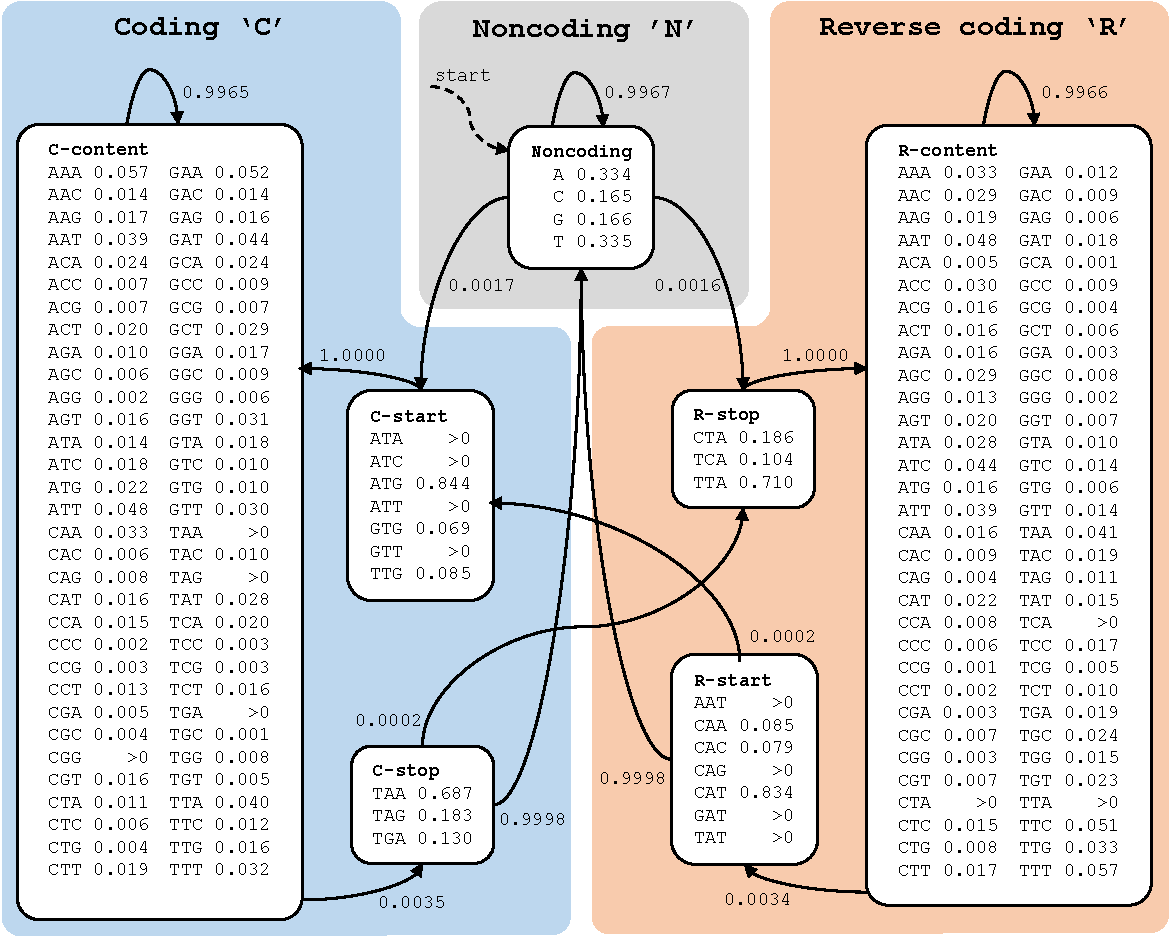
\includegraphics[width=\linewidth]{HMM_graph_cropped.pdf}
	\caption{Transition diagram and state emissions for our HMM for genome annotation by explicitly matching codons within coding areas, and enforcing certain start and stop codons. Transition and emission probabilities approximated by counting annotated data.}
	\label{fig:hmm_graph}
\end{figure}

All coding states in the model, only allow for three letter \emph{codon} outputs. This could be approximated by expanding every such codon emitting state to three letter emitting states. To only allow some codons, a combination af many three letter emitting states configurations in parallel could have been used. Such a model, that could express all those probabilities derived from counting occurrences would have to have nearly 500 states. 

To avoid such many states, we opted for this simple 7 state model. To complexity was then shifted towards the implementation of the viterbi algorithm, since it would need to accommodate variable length outputs. 


\section*{Approximating probabilities by counting occurrences}
Emission- and transitions probabilities was approximated by counting every occurrence of emission output or state change. The 68 possible emissions span a set of the single letters 'A', 'C', 'G', 'T' for noncoding, and the 64 three letter codon combinations hereof for coding regions. The states representing the start and stop codons seem to be from a very limited set of codons. The prior probabilities of starting in a certain state, $\pi$, was set to start in the noncoding, since nothing else has occurred in the dataset given. 


\section*{Decoding genomes}
The Viterbi algorithm has been tried implemted for decoding a genome with our HMM described above. But it seems that the probabilities for being in some conding states allways are lower than just staying in the noncoding state.


\section*{Performance}
Cross validation of our model has been tried. The overall idea is to devide the dataset into reasonable chunks, and then in turn not include a chunk when training/counting for the model. The achieved model can then be used on the excluded chunk to give a impression of performance when used on unseen data. The Approximate correlation Coefficient \emph{AC} can be used to compare genome annotations. 

Since we could not get our algorithm to guess on other than noncoding areas, then no results can be given.
\begin{table}
	\centering
	\caption{text}
	\label{tab:ac}
	\begin{tabular}{rccc}
		& \multicolumn{3}{c}{Approximate correlation coefficient} \\ 
		validation & C & R & Both \\ 
		\midrule
		Genome 1 &  &  &  \\ 
		Genome 2 &  &  &  \\ 
		Genome 3 &  &  &  \\ 
		Genome 4 &  &  &  \\ 
		Genome 5 &  &  &  \\ 
		Average & & & \\
	\end{tabular} 
\end{table}
	
\end{document}
